\documentclass[border=3pt]{standalone}
% Preâmbulo compartilhado pelos diagramas TikZ da aula 6 de IHC (Necessidades e Requisitos)
\usepackage[T1]{fontenc}
\usepackage[utf8]{inputenc}
\usepackage{lmodern}
\usepackage{amsmath}
\usepackage{xcolor}
\usepackage{tikz}
\usetikzlibrary{arrows.meta,angles,quotes,decorations.pathmorphing,calc,
                positioning,shapes.geometric,shapes.misc,backgrounds,fit,
                math}

% Paleta (mesma dos SVGs originais)
% Paleta da disciplina de IHC: acento roxo (#755099), da capa do livro.
% (o nome "dblue" é mantido para não alterar todos os diagramas)
\definecolor{dblue}{HTML}{755099}
\definecolor{dorange}{HTML}{B3541E}
\definecolor{dgreen}{HTML}{4A7C59}
\definecolor{dred}{HTML}{9C4B4B}
\definecolor{dcream}{HTML}{F4F1EA}
\definecolor{dshade}{HTML}{DDD7C9}

% Função gaussiana (não normalizada por padrão de escala visual)
\pgfmathdeclarefunction{gauss}{3}{%
  \pgfmathparse{1/(#3*sqrt(2*pi))*exp(-((#1-#2)^2)/(2*#3^2))}%
}

% Estilos comuns (prefixo d... para não colidir com chaves internas do pgf)
\tikzset{
  >={Stealth[length=2mm]},
  dguide/.style={gray!55, dashed, line width=0.4pt},
  daxis/.style={gray!60, line width=0.7pt, ->},
  dbody/.style={fill=black!3, draw=black!80, line width=1pt},
  dacc/.style={draw=dblue, line width=1pt},
  dlbl/.style={black!55, font=\small},
  dsub/.style={black!45, font=\footnotesize},
  dstate/.style={circle, draw=black!80, fill=dcream, line width=1pt,
                 minimum size=17mm, font=\large, inner sep=1pt},
  dobs/.style={circle, draw=black!80, fill=dshade, line width=1pt,
               minimum size=14mm, font=\large, inner sep=1pt},
  dbox/.style={rounded corners=2pt, draw=black!80, fill=dcream, line width=1pt,
               align=center, inner sep=6pt},
  dop/.style={circle, draw=black!80, fill=white, line width=1pt,
              minimum size=6mm, inner sep=0pt, font=\small},
  dtrans/.style={->, dblue, line width=1pt},
  dmeas/.style={->, dorange, line width=1pt},
  dcurve/.style={line width=1pt, dblue},
  dcurveb/.style={line width=1.4pt, dorange},
}

\begin{document}
\hyphenpenalty=10000 \exhyphenpenalty=10000 \tolerance=9999 \emergencystretch=3em
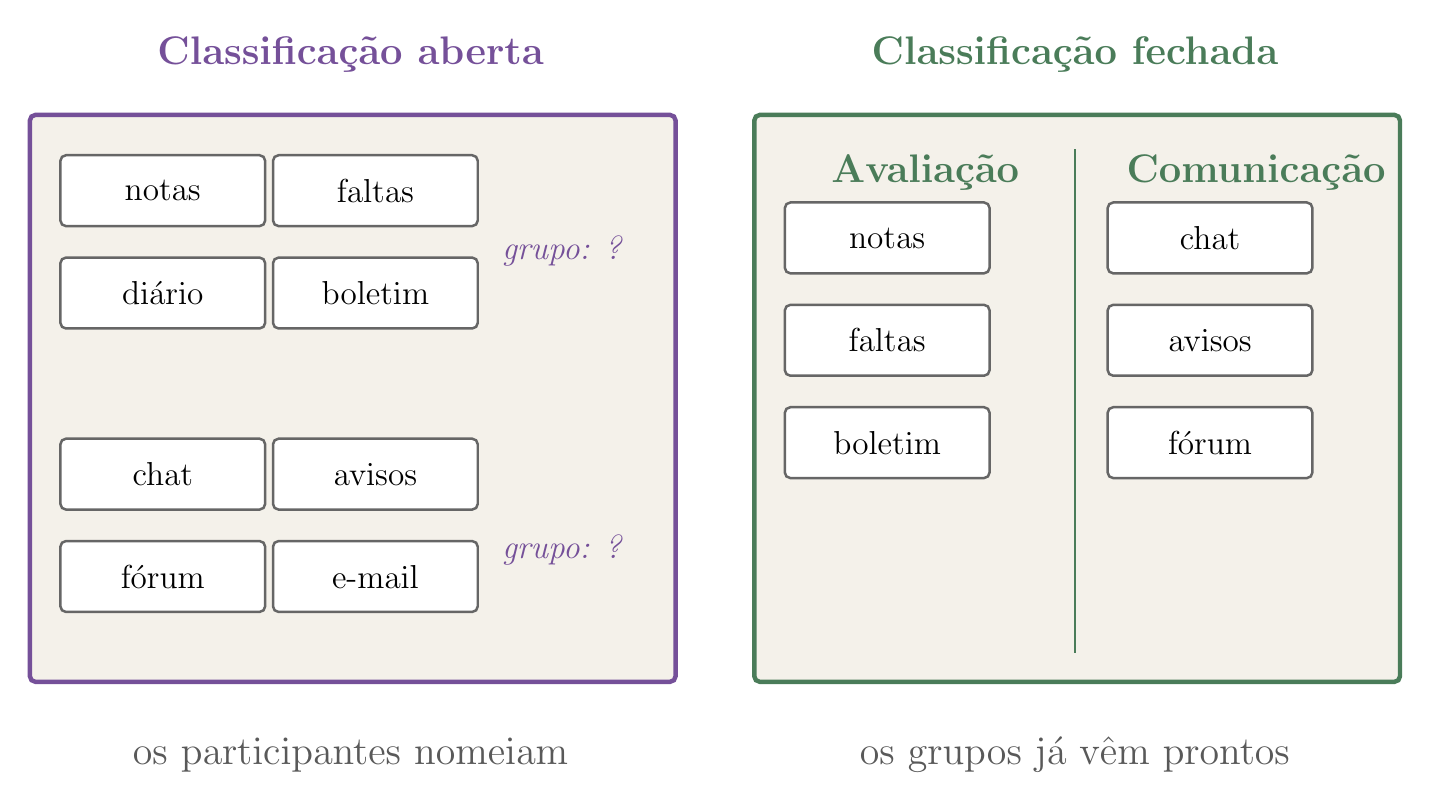
\begin{tikzpicture}[x=1cm,y=1cm]
  \tikzset{c/.style={draw=black!60, fill=white, rounded corners=2pt, minimum width=2.6cm, minimum height=0.9cm, font=\large, line width=0.9pt}}
  \tikzset{g/.style={dbox, minimum width=8.2cm, minimum height=7.2cm, line width=1.6pt}}
  \node[font=\Large\bfseries, dblue] at (4.1,8.4) {Classificação aberta};
  \node[g, draw=dblue, anchor=south west] at (0,0.4) {};
  \foreach \x/\y/\t in {0.4/6.2/notas, 3.1/6.2/faltas, 0.4/4.9/diário, 3.1/4.9/boletim, 0.4/2.6/chat, 3.1/2.6/avisos, 0.4/1.3/fórum, 3.1/1.3/e-mail} {\node[c, anchor=south west] at (\x,\y) {\t};}
  \node[font=\large\itshape, dblue, anchor=west] at (5.9,5.9) {grupo: ?};
  \node[font=\large\itshape, dblue, anchor=west] at (5.9,2.1) {grupo: ?};
  \node[font=\Large, black!65] at (4.1,-0.5) {os participantes nomeiam};
  \node[font=\Large\bfseries, dgreen] at (13.3,8.4) {Classificação fechada};
  \node[g, draw=dgreen, anchor=south west] at (9.2,0.4) {};
  \node[font=\Large\bfseries, dgreen] at (11.4,6.9) {Avaliação};
  \node[font=\Large\bfseries, dgreen] at (15.6,6.9) {Comunicação};
  \draw[dgreen, line width=1pt] (13.3,0.8) -- (13.3,7.2);
  \foreach \x/\y/\t in {9.6/5.6/notas, 9.6/4.3/faltas, 9.6/3.0/boletim, 13.7/5.6/chat, 13.7/4.3/avisos, 13.7/3.0/fórum} {\node[c, anchor=south west] at (\x,\y) {\t};}
  \node[font=\Large, black!65] at (13.3,-0.5) {os grupos já vêm prontos};
\end{tikzpicture}
\end{document}
